\documentclass[a4paper]{article}

%% Language and font encodings
\usepackage[english]{babel}
\usepackage[utf8x]{inputenc}
\usepackage[T1]{fontenc}

%% Sets page size and margins
\usepackage[a4paper,top=3cm,bottom=2cm,left=3cm,right=3cm,marginparwidth=1.75cm]{geometry}

%% Useful packages
\usepackage{amsmath}
\usepackage{graphicx}
\usepackage[colorinlistoftodos]{todonotes}
\usepackage[colorlinks=true, allcolors=blue]{hyperref}

\title{Actividad VIII}
\author{José Pablo Montaño De la Ree}
\date{ 12 de abril del 2018}

\begin{document}
\maketitle



\section{Introduccion}

En el universo de la fisica, siendo un poco más espesifico el de la dinamica, existen ciertos sucesos periodicos que se repiten en cuanto a su estado de movimiento como puede ser un resorte. Este tipo de movimiento es al cual se le considera un oscilador. Pues en esta ocacion se modelara un oscilador conocido como el oscilador de Van der Pol el cual tiene un amortiguamiento no lineal.
 \linebreak
 
 Este oscilador fue inicialmente propuesto por el ingeniero electrico Sueco Baltazar Van der Pol, el cual trabajaba en philips. El encontro unas oscilaciones estables a las cuales llamo oscilaciones relajadas las cuales son conocidas como un tipo de ciclo limite en circuitos electricos que usan tubos de vacio. 
 
 La ecuacion diferencial no lineal que se utiliza para modelar este fenomeno es la siguiente:
 
 \begin{figure}[ht!]
\centering
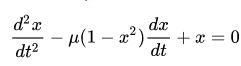
\includegraphics[width=0.3\textwidth]{E1.png}
\end{figure}

\section{ Modelo de Van der Pol y Exploración de las soluciones del modelo en el Espacio Fase}

Como ya se menciono anteriormente, existe una ecuacion que modela el oscilador de Van der Pol. Esta ecuacion tiene una caracteristica muy interesante, resulta ser que esta tiene un ciclo limite. Esto significa que todos los resultados caen detro de un espacio geometrico, se podria decir. Para comprobar esto se puede revisar que la ecuacion de Van der pol cumple con la ecuacion de Lienard para probar los ciclos limite. 
\linebreak

\subsection{Exploracion de soluciones}

Existen diferentes maneras de ver la ecacion de Van der Pol a travez de ciertas transformaciones que pueden permitir un modelado más sencillo de programar. Al Aplicar la siguiente transformacion

 \begin{figure}[ht!]
\centering
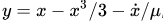
\includegraphics[width=0.3\textwidth]{T1.png}
\end{figure}

Se pueden onbtener los siguientes resultados para modelar la ecuacion de van der Pol. 

\begin{figure}[ht!]
\centering
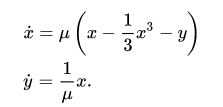
\includegraphics[width=0.3\textwidth]{Eq1.png}
\end{figure}

Sin embargo tambien se pueden obtener las siguientes ecuaciones como forma alternativa, las cuales seran las que se utilizaran para realizar el modelado en Jupyter lab como se muestra a continuacion.


\begin{figure}[ht!]
\centering
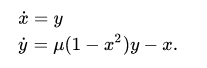
\includegraphics[width=0.3\textwidth]{Eq2.png}
\end{figure}

\begin{verbatim}

def vectorfield(w, t, p):
    """
   
   Vector Vanderpol
   
    Arguments:
        w :  vector of the state variables:
                  w = [x,y]
        t :  time
        p :  vector of the parameters:
                  p = [u]
    """
    X, Y = w

    # Create f = (x',y'):
    f = [Y,
         p*(1.0 - (X**2.0))*Y -X]
    return f

\end{verbatim}

\section{ Resultados y Discucion}


Los resultados obtenidos del modelado fueron las siguientes graficas. 

Primero veamos las graficas de como varia X respecto a Y


\begin{figure}[ht!]
\centering
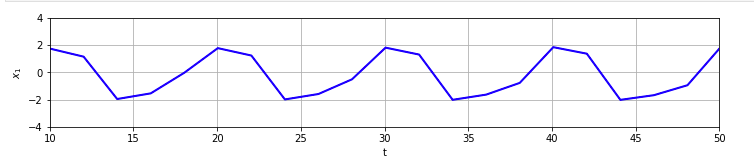
\includegraphics[width=0.3\textwidth]{G1.png}
\end{figure}

\begin{figure}[ht!]
\centering
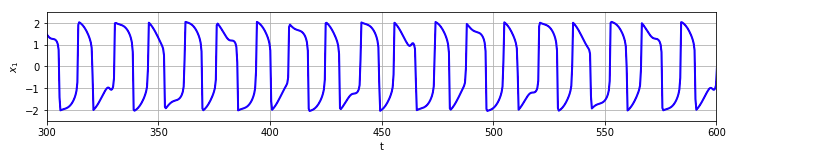
\includegraphics[width=0.3\textwidth]{G2.png}
\end{figure}

Notse que la variacion que se presenta es de una forma sinoildal y aunque de la segunda  imagen podria pensarse que existe suficiente suavidad para un modelado senoidal, en la primera imagen se revelan picos que inpiden el uso de este modelo.
\linebreak

Ahora, grafiquemos nuestros componentes X y Y respecto al tiempo para poder observar como se comportan y poder descubrir los ciclos limite.

\begin{figure}[ht!]
\centering
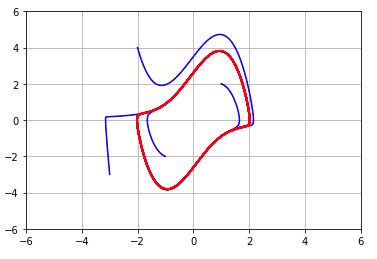
\includegraphics[width=0.3\textwidth]{G3.png}
\end{figure}

\begin{figure}[ht!]
\centering
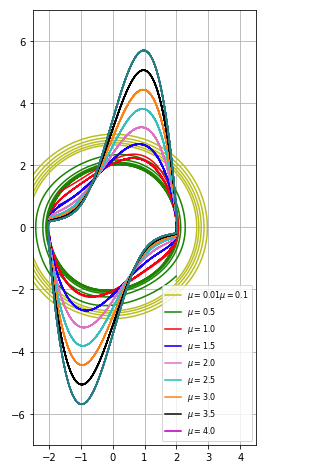
\includegraphics[width=0.3\textwidth]{G4.png}
\end{figure}

\newpage

Notese que se forma una superficie espesifica, esta superficie es a la que se conoce como ciclo limite.

\section{Concluciones}

Existen cituaciones fisicas reales como el oscilador de Van der pol que requieren ser modelados de fomra computacional para tener una mejor apreciacion de estos. En el caso espesifico de la ecuacion de Van der Pol, podemos asegurar que existe un cilo limite al mirar las graficas.

\section{Referencias}

Wikipedia. (2018). Van der Pol oscillator. 12 de Abril del 2018, de Wikipedia Sitio web: 
\begin{verbatim}
https://en.wikipedia.org/wiki/Van_der_Pol_oscillator
\end{verbatim}


\end{document}